\section{Key Network Parameters and Derived Cost Functions}
\label{ch1:sec:key-network-parameters}

In literature (see Chapter \ref{ch-review}), two distinct approaches have emerged to quantitatively improve the performance of a system:
either cost is reduced or utility is maximised.
Both approaches rely on a mathematical explanation of underlying features that relate to performance of the system.
To recap; utility functions are maximised since they explain how beneficial a system state is, whereas cost should be minimised since they entail a suboptimal system performance.
The choice for this piece of work was to associate key network parameters to tailored cost functions, with the reason that a cost can be minimised to a finite value, i.e. zero.
Utility maximisation on the other hand is a mathematically unbound problem that may reach a maximum, yet this maximum can only be approximated though game theoretic approaches like Pareto- or Nash-Optimality.
In other words, solutions to a cost function where the resulting cost is zero, are by definition optimal solutions, whereas a utility functions can have multiple maxima where optimality classification of these solutions is inherently more difficult.
To illustrate this fact, an arbitrary utility function, $\zeta_{u}(x)$, and an arbitrary (and unrelated) cost function, $\zeta_{c}(x)$, have been plotted in Figures \ref{ch1:subfig:sketch-utility} and \ref{ch1:subfig:sketch-cost}, respectively.

\begin{figure}\centering
	\subfloat[Sample utility function]{%
		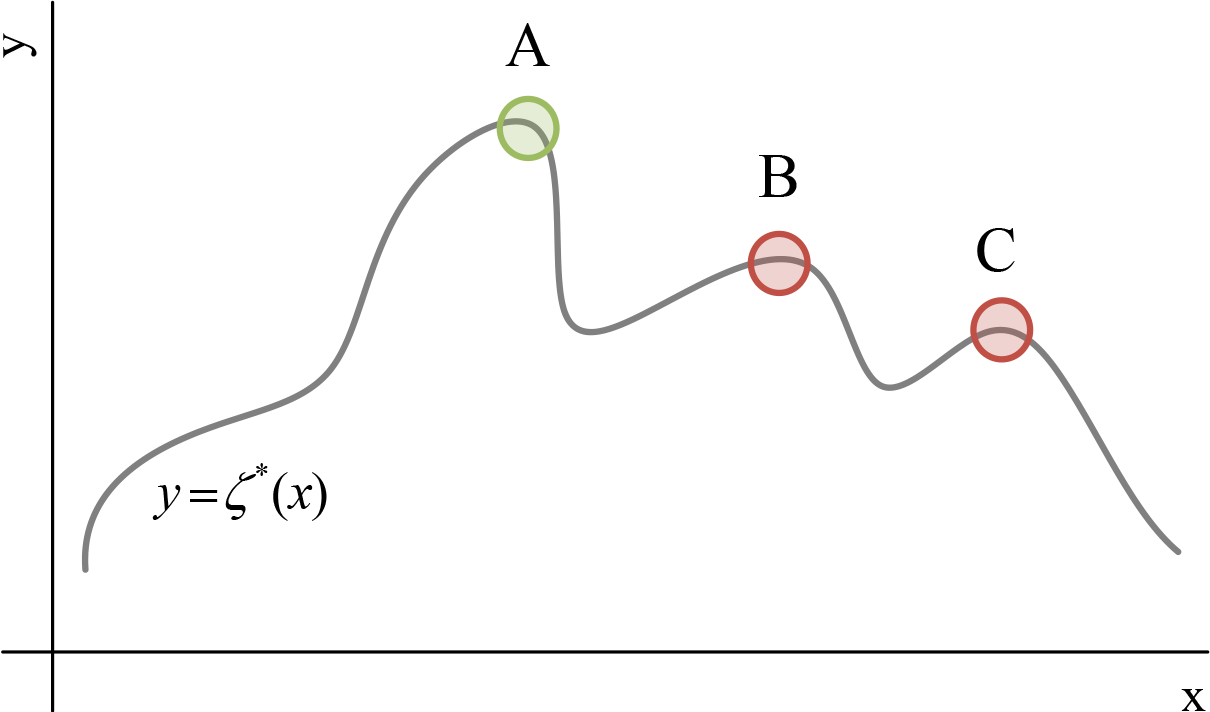
\includegraphics[width=0.45\textwidth]{_chapter1/fig/sketch-utility}%
		\label{ch1:subfig:sketch-utility}%
		}
	\hspace{5mm}
	\subfloat[Sample cost function]{%
		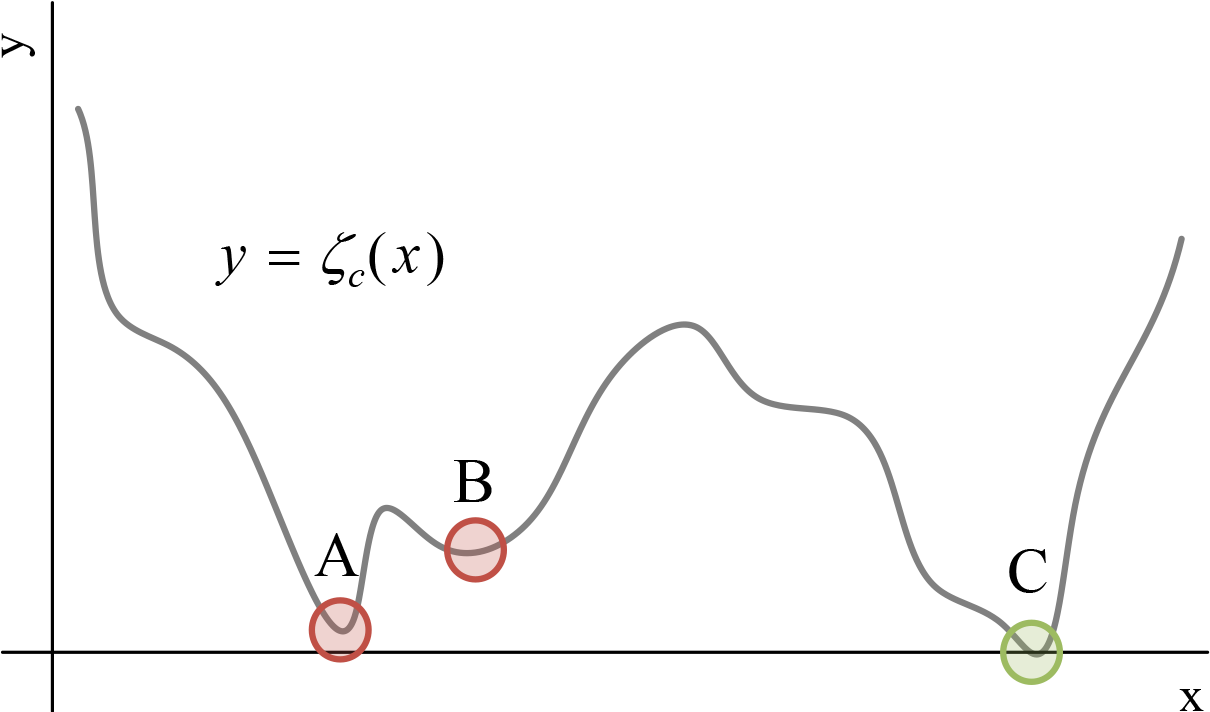
\includegraphics[width=0.45\textwidth]{_chapter1/fig/sketch-cost}%
		\label{ch1:subfig:sketch-cost}%
		}
	\caption{Benefit of using cost function over utility function}
	\label{ch1:fig:sketch-utility-vs-cost}
\end{figure}

These two figures illustrate how the peaks of the utility function are at different, large values of $y$, and the troughs of the cost function tend towards zero.
Both peaks or minima are found using solving algorithms; the most common mathematical solvers are the Gradient Descend Method, Newton-Raphson Method, and Active Set Method.
If the cost or utility function is nonlinear or the system's gradient function can only be approximated more sophisticated algorithms had to be used, e.g. Mixed-Integer Linear Programming, Sequential Quadratic Programming (SQP), Genetic Algorithm, Particle Swarm Optimisation or the Interior Point Method.
Depending on the starting conditions of those solvers, i.e. the initial values for $x$, different maxima or minima (i.e. points $A$, $B$ or $C$) may be found.
In the example above, the best solution for $\zeta_{c}(x)$ is at point $A$, whereas the best solution for $\zeta_{c}(x)$ is at point $C$.
Whilst point $A$ represents the highest utility, it is difficult to determine whether this maximum is a most optimal solution since utility is inherently unbounded, i.e. $\zeta_{c}(x) \in (-\infty, \infty) \forall x$.
For the cost function on the other hand, point $C$ is represents an absolute minimum and optimal solution since the cost function's range is bounded to be greater or equal to zero, i.e. $\zeta_{c}(x) \geq 0 \forall x$.
Therefore, the cost's proximity to zero can directly indicate the system performance (whilst a utility's proximity to infinity would not make sense).

With this in mind, the key network parameters are explained and the corresponding cost functions are defined next.
The choice of parameters is virtually inexhaustible since one could treat every single current, voltage or phase angle as a potential indicator for network performance.
In reality however (and particularly in the context of NTVV), a power distribution network can only be observed at a limited number of points.
Here, these points were at the substation and the ESMU's Point of Common Coupling (PCC).
Therefore, all derived network parameters that are based on these measurements are treated as ``realistic parameters''.
It is however worth mentioning, that for the work presented in this chapter, all realistic parameters are extracted from power flow simulations.

In those simulations of power distribution networks (i.e. in OpenDSS), a system of equations that captures nodal power flow is solved.
In the IEEE LV Test Case, there are 906 three phase buses, resulting in a total of 2718 nodes, for which complex currents and voltages can be obtained.
This abundance of values means that a lot of additional parameters can be considered.
Yet those parameters cannot easily be obtained in reality, which is why they are referred to as ``theoretical parameters''.
Due to the high abundance of these theoretical parameters, the impact of some of these parameters on network performance is quite limited.
Therefore the set of theoretical parameters, that were used in this piece of work, was chosen based on their importance and impact on actual network operation.

A list of all realistic and theoretical key network parameters\footnote[1]{A key network parameter is marked with a dagger ($\dagger$) if it is a theoretical parameter that can only be extracted form power flow simulations.} is presented below.

\begin{itemize}
	\item Voltages at substation transformer's secondary winding
	\item Voltages at ESMU's PCC
	\item Voltages at customer lateral$^{\dagger}$
	\item Total power flow
	\item Substation line utilisation
	\item Maximum line utilisation$^{\dagger}$
	\item Distribution losses$^{\dagger}$
\end{itemize}

In the following subsections, the formulation of all key network parameters' associated cost functions is presented.

\subsection{Voltages at substation}
\label{ch1:subsec:voltages-at-substation}

In UK LV distribution networks, substations supply power to a feeding cable.
These substations provide the link from MV distribution networks, which operates at 11kV P2P, to the LV distribution network, which operates at nominal 230V P2N (i.e. 400V P2P).
If the substation transformer was an ideal transformer, then the voltage measured at its secondary winding would remain constant with changing load.
In reality however, the internal losses (e.g. conductive losses and magnetic leakage) lead to a drop in voltage as load increases.
Therefore, any deviation from the substation's nominal voltage may be an indicator of suboptimal network operation.

Let the substation voltage for a single phase voltage be defined as $v_{ss,\phi}(t)$, where $p$ is the phase number and $t$ the time at which the measurement was taken.
Then the resulting substation voltage vector $\textbf{v}_{ss}(t)$ (where $v_{ss,\phi}(t) \in \textbf{v}_{ss}(t)$) can be fed into a deviation cost $\zeta_\text{voltage}(\textbf{v}_{ss}(t))$ to assess the cost of substation overloading.
This cost is defined for any voltage vector (here $\textbf{v}(t)$) as:

\begin{equation}
\begin{split}
	\zeta_\text{voltage}(\textbf{v}(t)) :=& \sum_{\phi=1}^{\Phi}{\begin{cases}
		\zeta_h(v_{\phi}(t)) & \text{if } V_{ss} \leq v_\phi\\
		\zeta_l(v_{\phi}(t)) & \text{otherwise}\\
	\end{cases}} \forall t\\
	&\text{ where } \Phi \in \mathbb{Z}^{>0}
\end{split}
\label{ch1:equ:voltage-deviation}
\end{equation}

In this voltage cost function, $\Phi$ represents the number of phases (i.e. $\Phi = 3$), and $\zeta_h(v)$ and $\zeta_l(v)$ are two functions that convert a single voltage value, i.e. $v_p$, into a normalised positive cost based upon the direction of voltage deviation.
E.g. if the voltage $v_p$ is greater than or equal to the nominal substation voltage, $V_{ss}$, then the result from $\zeta_h(v)$ is used as a cost; otherwise the result from $\zeta_l(v)$ is used.
In order to define these two functions, the corresponding high and low voltage thresholds, respectively $V_h$ and $V_l$, are introduced.
With those high and low voltage bands, $V_{ss}$ has to be chosen in order to satisfy the following inequality:

\begin{equation}
	V_l < V_{ss} < V_h
\end{equation}

For the presented work, these two voltage thresholds are based on the UK's nominal LV voltage range of +10\% -6\% around $V_n$, i.e. 230V P2N.

\begin{equation}
	\zeta_h(v) := \alpha \left|\frac{v-V_{ss}}{V_h-V_{ss}}\right|^{\beta}
	\label{ch1:equ:high-voltage-threshold-cost-complete}
\end{equation}

\begin{equation}
	\zeta_l(v) := \alpha \left|\frac{V_{ss}-v}{V_{ss}-V_l}\right|^{\beta}
	\label{ch1:equ:low-voltage-threshold-cost-complete}
\end{equation}

In this context of defining $\zeta_{voltage}$, the variable $\alpha$ is used as the functions' linear weight that scales the corresponding cost, and the variable $\beta$ linearly increases the functions' gradients as voltage continues to deviate.
More specifically, $\alpha$ determines the value of the functions at voltages $V_l$ and $V_h$, where $\alpha \in \mathbb{R}^{>0}$; for example, when $\alpha = 1$, then $\zeta_{h}(v_l) = 1$.
$\beta$ on the other hand may take any value in the range of $\mathbb{R}^{>2}$, to assure a continuously differentiable cost function.
Both $\alpha$ and $\beta$ were treated as constants and, for the scope of this work, set to $1$ and $2$, respectively.
Substituting these values into Equations \ref{ch1:equ:high-voltage-threshold-cost-complete} and \ref{ch1:equ:low-voltage-threshold-cost-complete}, simplifies the high and low cost functions to:

\begin{equation}
	\zeta_h(v) := \left|\frac{v-V_{ss}}{V_h-V_{ss}}\right|^{2}
	\label{ch1:equ:high-voltage-threshold-cost-simple}
\end{equation}

\begin{equation}
	\zeta_l(v) := \left|\frac{V_{ss}-v}{V_{ss}-V_l}\right|^{2}
	\label{ch1:equ:low-voltage-threshold-cost-simple}
\end{equation}


Since voltage levels drop continuously along a purely consumptive feeder, substations may boost the voltage above the nominal LV voltage level, yet keep it below the upper voltage threshold.
The behaviour of boosting $V_{ss}$ on the cost function $\zeta_\text{voltage}(\textbf{v})$ is shown below (here $\Phi = 1$).

\begin{figure}\centering
	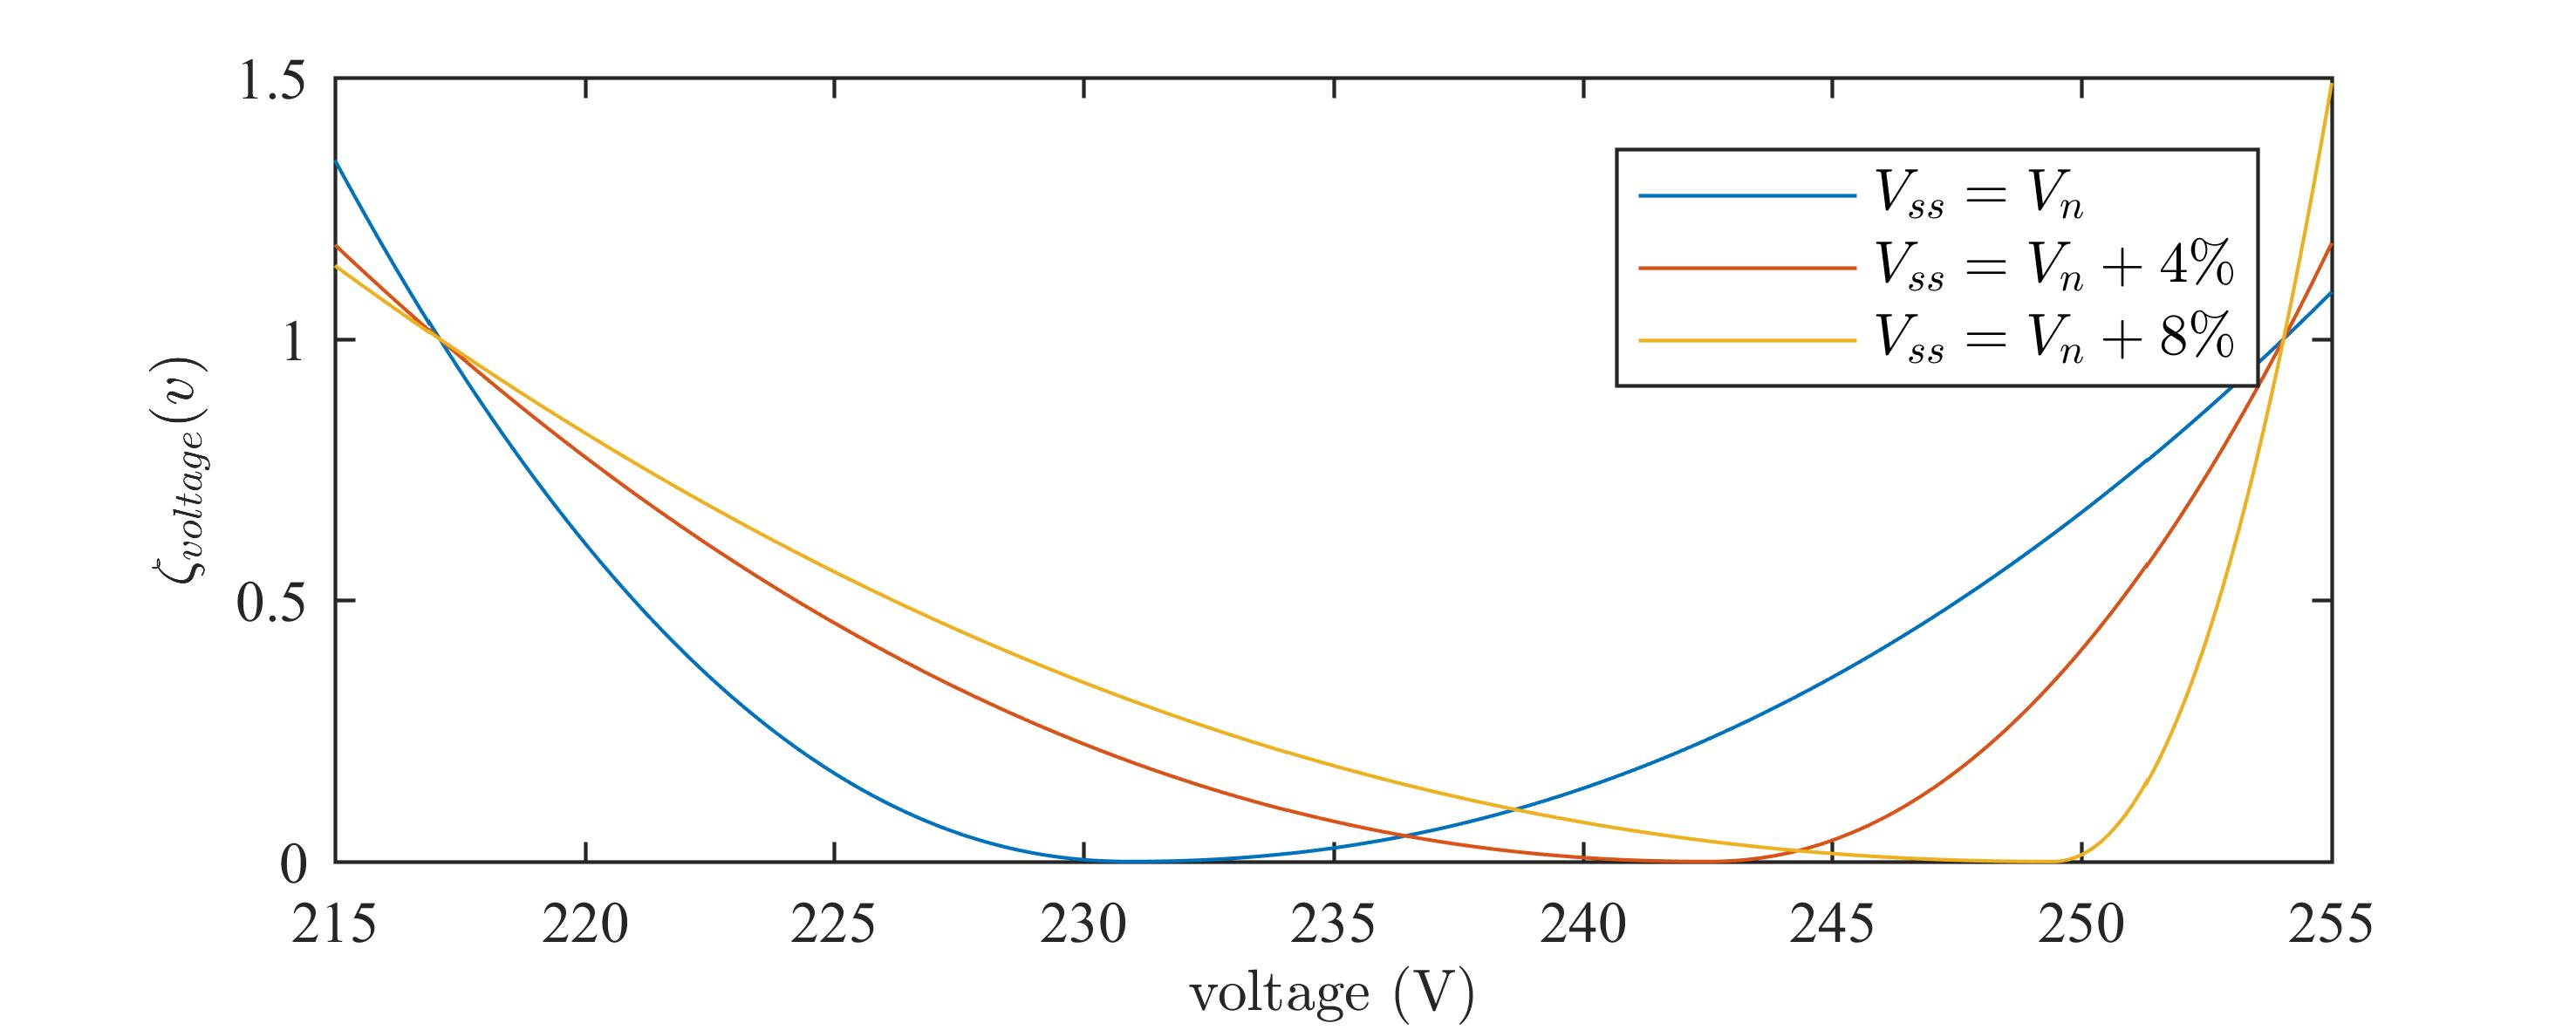
\includegraphics{_chapter1/fig/voltage-deviation}
	\caption{Cost function $\zeta_\text{voltage}(v_\phi)$ values for different substation voltages}	
	\label{ch1:fig:voltage-deviation}
\end{figure}

It can be seen that the cost at the high and low voltage thresholds equates to one, and to zero at the set substation voltage.
When boosting this voltage, $V_{ss}$, only the zero intersection is moved, whereas the high and low voltage crossings remain unchanged.
In Figure \ref{ch1:fig:voltage-deviation}, this behaviour is demonstrated by boosting $V_{ss}$ by +4\% and +8\%.

\subsection{Voltages at ESMU's PCC}
\label{ch1:subsec:voltages-at-esmu}

At the ESMU's PCC, it is connected to all three phases of the feeding cable.
The location of this PCC is at some distance from the substation or simply ``down stream'' the feeder.
Where to connect the ESMU, in order to achieve a best possible network impact, is explained in Section \ref{ch1:sec:data-and-network-models}.
Ignoring the exact ESMU location, voltage along the line, i.e. from the substation to its PCC, will change and most likely drop.
The reason behind this effect is due to resistive and inductive losses in the distribution lines.
These losses are amplified with proximity to the substation, since load currents are aggregated.
For purely consumptive loads, and particularly under heavy load conditions, this voltage may at some stage drop below the low-voltage threshold.
As mentioned in literature, this threshold is an operational constraint of LV networks and must not be violated to assure correct appliance operation and prevent financial penalisation.

In order to mitigate this voltage drop, power is injected into the feeder at the ESMU's PCC.
Doing so boosts the voltage at that location since the portion of the load current that would normally be supplied by the substation is now delivered by the ESMU.
The effect of this power injection is sketched in the figure below.

\begin{figure}\centering
	\subfloat[Voltage drop along feeder without ESMU intervention]{%
		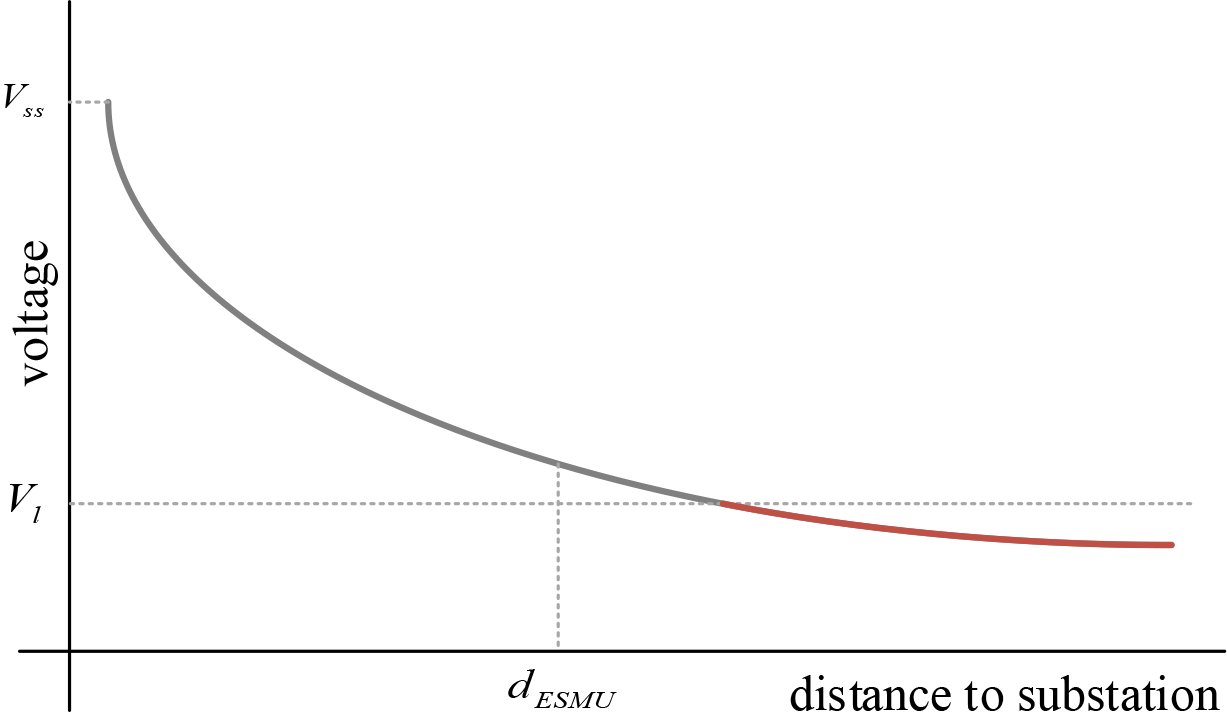
\includegraphics[width=0.45\textwidth]{_chapter1/fig/sketch-voltage-esmu-normal}%
		\label{ch1:subfig:sketch-voltage-esmu-normal}%
		}
	\hspace{5mm}
	\subfloat[Voltage drop along feeder with ESMU intervention]{%
		
\includegraphics[width=0.45\textwidth]{_chapter1/fig/sketch-voltage-esmu-boost}%
		\label{ch1:subfig:sketch-voltage-esmu-boost}%
		}
	\caption{Benefits of ESMU power injection on the voltage drop along the feeder}
	\label{ch1:fig:sketch-voltage-esmu}
\end{figure}

In Figure \ref{ch1:subfig:sketch-voltage-esmu-normal}, an expected voltage drop along the feeder is sketched, where the down stream feeder section's voltage dropped below $V_l$.
In contrast, Figure \ref{ch1:subfig:sketch-voltage-esmu-boost} shows how the ESMU's intervention can alleviate some load and raise the trailing voltage levels to a level above $V_l$.

This realistic key network parameter is translated into a cost function, since the P2N voltage at the ESMU's PCC can be measured quite easily.
To do so, the three-phase PCC voltage, $\textbf{v}_{ESMU}(t)$ (where $v_{ESMU,\phi}(t) \in \textbf{v}_{ESMU}(t)$), is used in Equation \ref{ch1:equ:voltage-deviation}; the same cost used for the substation transformer's secondary voltage.
Therefore, the resulting cost can be formulated as $\zeta_\text{voltage}(\textbf{v}_{ESMU}(t))$.

\subsection{Voltages at customer laterals}
\label{ch1:subsec:voltages-at-customers}

As mentioned in Chapter \ref{ch-introduction:sec:overview}, the allowable voltage range at customers is defined by the Electricity Safety, Quality and Continuity Regulations (ESQCR).
Monitoring those voltages in real-time to assure they obey these regulations is costly, and therefore they are left unmonitored.
Ultimately, when it comes to voltage level correction, only substation voltage levels and customer voltage levels need to be controlled.
This fact is to assure proper transformer operation (e.g. to maximise its lifespan) and to prevent penalisation due to customer voltage violation (i.e. fining according to the ESQCR).
As explained in Section \ref{ch1:subsec:voltages-at-esmu}, ESMU can impact voltage levels for all customers but, as mentioned above, these voltage levels cannot be measured in reality.
In simulations however, all loads' voltages can be extracted with ease, which is why they are included but treated as theoretical key network parameters.

To illustrate this load voltage drop, a snapshot OpenDSS simulation was run on the IEEE LV Test Case with all load powers set to a high value of 8kW\footnote[1]{Whilst historic and recent loads may reach values of this magnitude quite seldom, future customer demand with the aggregated effect home-charging of EVs may indeed yield extreme scenarios like this.}.
In the following plot, the magnitude of the load bus voltages against the distance between the corresponding load and its feeding substation was drawn.

\begin{figure}\centering
	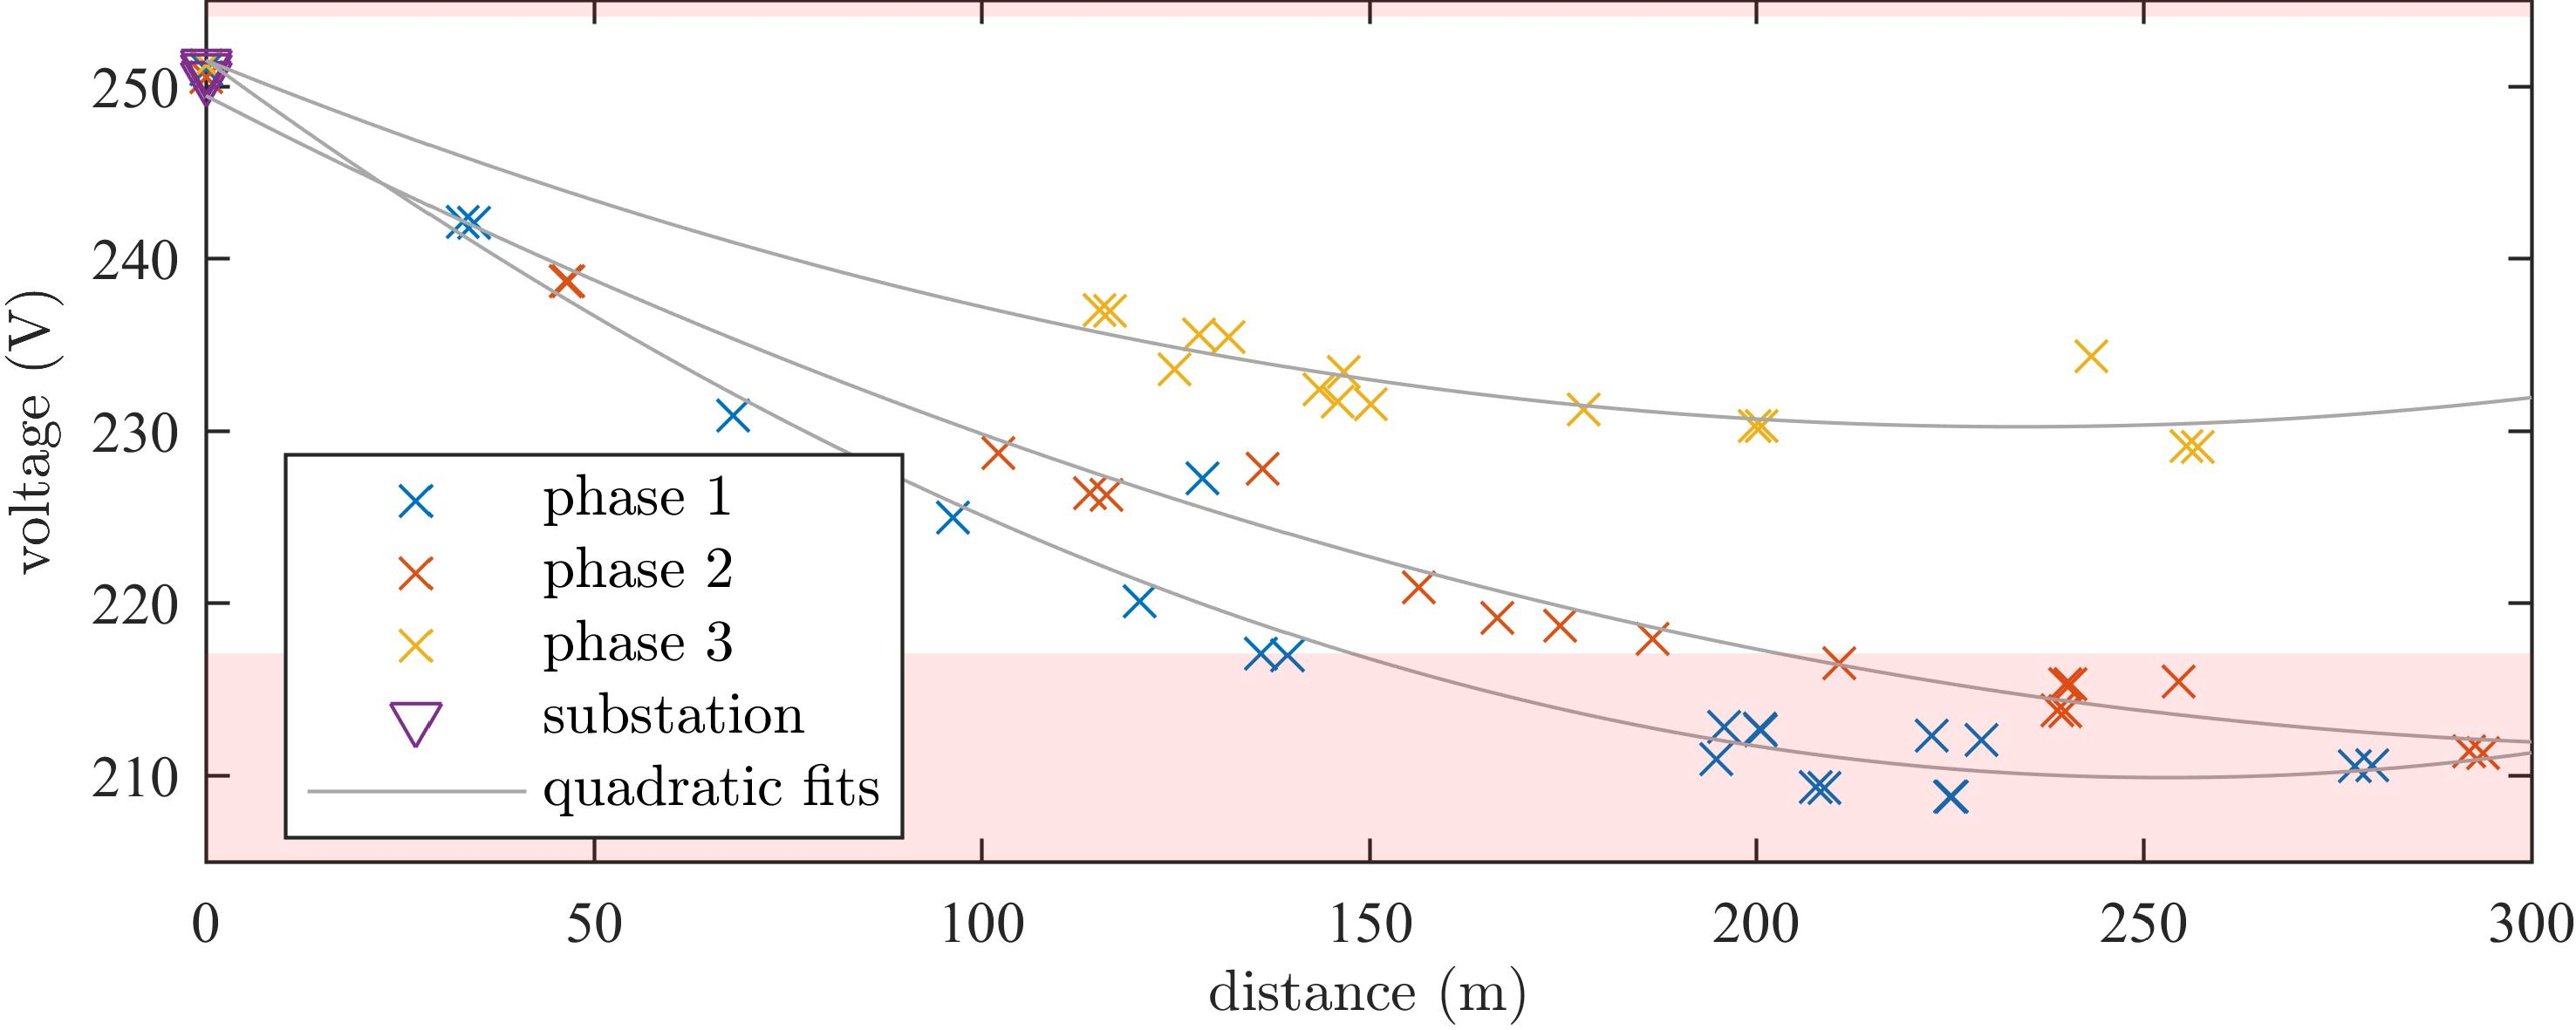
\includegraphics{_chapter1/fig/voltage-drop-for-loads-along-feeder}
	\caption{Voltage at the loads in the IEEE LV Test Case network for a total load of 440kVA against distance between the corresponding load and substation: for the quadratic fit $R^2=58.76\%$}
	\label{ch1:fig:voltage-drop-for-loads-along-feeder}
\end{figure}

In this Figure \ref{ch1:fig:voltage-drop-for-loads-along-feeder}, two observations can be made.
For one, it can be seen that phases are significantly unbalanced.
Secondly, customers further than 200m from the substation experience low-voltage events (for this particular scenario).
As already proposed in the previous section, ESMU aims to avoid these voltage violations, but the number of loads would add significant computational burden on the any used solving algorithm.

To address this problem, the previously defined voltage cost function (i.e. Equation \ref{ch1:equ:voltage-deviation}) is expanded.
Rather than including the cost for every single customer's voltage deviation, only the worst deviation is used.
By limiting this number, solvers need not consider such a large number of parameters and only focus on the worst network parameter.
This focus is of particular need if the impact of the ESMU on some customers' voltages is relatively low, since the aggregate cost would otherwise cloud the impact on those individual voltages.
For this work, the customer (or load) voltage is defined as $\textbf{v}_{load}(t)$ (where $v_{load,i,\phi} \in \textbf{v}_{load}$) and used in the new cost function, $\zeta_\text{load voltage}(\textbf{v}_{load}(t))$, as such:

\begin{equation}
\begin{split}
	\zeta_\text{load voltage}(\textbf{v}(t)) := \max_{i,\phi}{\zeta_\text{voltage}(v_{i,p}(t))} \\
	\text{ where } i \in \{1, \dots I\} \text{ and } \phi \in \{1, \dots, \Phi\} \text{ and } I \in \mathbb{Z}_{>0} \text{ and } \Phi \in \mathbb{Z}_{>0}
\end{split}
\label{ch1:equ:load-voltage-deviation}
\end{equation}

\subsection{Total power flow}
\label{ch1:subsec:total-power-flow}

Beside having to keep voltages within their specified operational boundaries, DNOs want to make sure that the distribution network operates in an efficient and ideal manner.
Determining how ideal a three-phase network operates can be done by e.g. assessing the balance of the network's phases.
The frequently neglected disturbance of unbalanced phases may not have an immediately associated impact on the network's customers, but the negative long term effects (e.g. asymmetric load on transformers, rotating machines and increased neutral current) must be addressed since they weaken the network's infrastructure.

The choice of how customers are connected to LV feeders in the UK makes phase unbalance a more dominant problem than one might have thought.
Customers in urban UK distribution networks have a single-phase link to the three-phase feeder line.
The link is established by connecting their supply cables or ``laterals'' between a phase and the neutral conductor.
In the UK, the phase allocation for each customer has been random, in order to distribute load as evenly as possible across all three phases.
In theory, this approach should assure a more or less balanced three-phase load, yet in reality this is not the case.
Even if the number of customers on each phase was the same for all three phases, the probability that all customers' load profiles are identical is very low.
Therefore, the likeliness of LV distribution feeders in the UK to be unbalanced is very high.

Since substation monitoring is capable of providing three-phase power measurements, they are used as realistic key network parameters, and summarised in a substation power vector $\textbf{s}_{ss}(t)$.
Deriving phase unbalance from these three-phase sub is done by following the American National Standards Institute (ANSI) definition of phase unbalance \cite{ANSI-MB-1-2011}.
The standardised Unbalance Factor (UF) is defined as:

\begin{equation}
	\text{UF}(\textbf{x}) := \frac{\max_n |\bar{\textbf{x}} - x_n|}{\bar{\textbf{x}}}
	\label{ch1:equ:unbalance-equation}
\end{equation}

Here, $\textbf{x}$ is a three phase vector, where $x_n \in \textbf{x} \text{ for } n=[1, 2, 3]$.
$x_n$ may be a voltage, current or power measurement per phase, but for context of this work $x_n$ was chosen to be the power flow into the network.
For clarity, the notation $\bar{\textbf{s}}$ is used to define the mean of all three phase values.
The mean's definition is give below:

\begin{equation}
	\bar{\textbf{x}} := \frac{1}{3}\sum_n^3{x_i}
\end{equation}

From the substation monitoring, a three-phase substation power vector, $\textbf{s}_{ss}(t)$ (where $s_{ss,\phi} \in \textbf{s}_{ss}$), is used and the network's phase unbalance can be calculated.
Since this forms another realistic key network parameter, the UF in Equation \ref{ch1:equ:unbalance-equation} was formulated into a cost function, too.
The resulting cost function $\zeta_\text{unbalance}(\textbf{s}_{ss})$ is defined as:

\begin{equation}
	\begin{split}
		\zeta_\text{unbalance}(\textbf{s}(t)):=&\text{UF}(\textbf{s}(t)) - 1 \forall t\\
		=&\frac{\max_p\left|\overline{\textbf{s}(t)} - s_{p}(t)\right|}{\overline{\textbf{s}(t)}} \forall t\\
		=&\frac{\max_p\left|\left(\frac{1}{P}\sum_p^P{s_{p}(t)}\right) - s_{p}(t)\right|}{\frac{1}{P}\sum_p^P{s_{p}(t)}} \forall t\\
		&\text{where } p \in [1, 2, \dots P]
	\end{split}
	\label{ch1:equ:unbalance-cost}
\end{equation}


The minimum value of $\text{UF}(\textbf{s}_{ss})$ is one.
Therefore an adjustment was required so that a perfectly balance network would result in an $\text{UF}(\textbf{s}_{ss})$ of zero.
An illustration how this cost function is provided in the Figure \ref{ch1:fig:power-unbalance}, as shown below.

\begin{figure}\centering
	
\includegraphics[width=5cm]{foo}
	\caption{Sample network imbalance for different phase loadings as defined in ANSI/NEMA MG 1-2011}
	\label{ch1:fig:power-unbalance}
\end{figure}

Here, it can be seen how $\zeta_\text{unbalance}(\textbf{s})$ varies with an increasing separation of the three phases' power values.

Additionally, to assess the effective utilisation of the power distribution network, the Power Factor (PF) divergence is also addressed.
PF is the ratio between the supplied active and apparent power.
It therefore gives an indication of how much ``good''\footnote[1]{Reactive power is used to maintain magnetic fields in rotating machines, yet this can be supplied by local reactive power compensators and thus need not occupy otherwise free power transmission resources.} power is being consumed by the system.
Experts would agree that keeping the PF of a system close to unity indicates that the system only draws active power and therefore is using the least amount of power transmission resources.
In order to asses the proximity to unity PF a PF cost function, $\zeta_{PF}(\textbf{s}_{ss}(t))$, is defined a power vector as input:

\begin{equation}
	\zeta_\text{PF}(\textbf{s}(t)):= \sum_{\phi=1}^{\Phi}\frac{\text{Re}(s_\phi(t))}{|s_\phi(t)|} - 1 \forall t \text{ where } s_\phi(t) \in \textbf{s}(t) \text{ and } \Phi \in \mathbb{Z}^{>0}
\label{ch1:equ:power-factor}
\end{equation}

Here, deviating from a unity PF per phase increases the associated cost, whilst achieving a perfect PF for each phase results in a total cost of zero.

Lastly, the already mentioned neutral current is also a result of both three-phase unbalance and non-unity PF.
Since all three phases are $120^\circ$ out of phase, the sum of instantaneous powers should equate to zero.
This would result in no neutral current flowing in the system.
However, in an unbalanced system the power transmitted through the neutral conductor deviates significantly from zero.
This situation is amplified since power distribution cables often use neutral conductors with significantly smaller diameter than those conductors used for the lines.
Therefore, any additional power flow in this neutral conductor will deviate neutral voltages from zero volts and it could also exhaust the conductor's power carrying capacity, making the system more prone to failures.
To address this last point, and before dealing with line utilisation, a final cost function that deals with the neutral loading $\zeta_{neutral\;\;load}(\textbf{s}_{ss}(t))$ is defined as follows:

\begin{equation}
	\zeta_\text{neutral load}(\textbf{s}(t)) := \left|\sum_{\phi=1}^{\Phi} s_\phi(t)e^{\frac{j2\pi\phi}{\Phi}}\right| \text{ where } \textbf{s}(t) = (s_\phi(t)) \text{ and } \Phi \in \mathbb{Z}_{>0}
\label{ch1:equ:neutral-load}
\end{equation}

For $\zeta_{neutral\;\;load}(\textbf{s}_{ss}(t))$, each phase power, $s_{ss,\phi}(t)$, is therefore rotated by an integer multiple of $120^\circ$ before adding them to obtain the neutral load vector.
The magnitude of this apparent power vector is the size of the load in the neutral conductor.

\subsection{Substation line utilisation}
\label{ch1:subsec:substation-line-utilisation}

Although phase unbalance deteriorates the efficiency and life expectancy of three-phase network assets, high power demand puts strain on the physical cables themselves.
This is due dominantly due to resistive and inductive losses heating the cables, and bringing them closer to their operational limits.
Therefore, cables have an assigned thermal rating which must not be exceeded to prevent permanent cable damage or network failures.
At substation level, to prevent over-currents, fuses or reclosers are installed that will disconnect the network under fault or high demand conditions.
To quantify whether the substation fuse is approaching its tripping point, its nominal rating is used as reference.

For the context of this work, this nominal fuse rating, $i_{fuse}$, is a fixed value for the fuse at the substation and must not be exceeded.
Using the three-phase current vector from substation monitoring, $\textbf{i}_{ss}(t)$ (where $i_{ss,\phi}(i) \in \textbf{i}_{ss}(t)$) a cost function, $\zeta_\text{fuse utilisation}(\textbf{i}_{ss}(t))$, can be defined as follows:

\begin{equation}
	\zeta_\text{fuse utilisation}(\textbf{i}(t)) :=%
	\left|\frac{\sum_{\phi=1}^{\Phi}{i_\phi(t)}}{I_\text{fuse}}\right|^2%
	\text{ where } \phi \in \{1, \dots, \Phi\}%
	\text{ and } \Phi \in \mathbb{Z}_{>0}
	\label{ch1:equ:fuse-utilisation}
\end{equation}

A plot has been included in the below figure, which illustrates how this quadratic cost behaves as substation current increases.

\begin{figure}
	
\includegraphics[width=5cm]{foo}
	\caption{Cost of line or fuse utilisation against network current}
	\label{ch1:fig:fuse-utilisation}
\end{figure}

For this simple case, the substation line rating was set as $i_{fuse}=400\text{A}$, and the total substation current is the sum of all three phase currents.

\subsection{Maximum line utilisation}
\label{ch1:subsec:maximum-line-utilisation}

Similar how voltage levels at all customers are theoretical key network parameters, currents in all lines are key network parameters, too.
Optimising the aforementioned current at substation level would prevent unintentional feeder disconnection and equipment damage, yet lines' ratings impose distributed limits, too.
Moreover, as feeder cables are not of a singly type of cable.
For instance, the main three-phase wire must to be sufficiently scaled to deliver several 100s of Amperes to a collection of customers, whilst branches with a few loads may only experience 10s of Amperes worth of current.
Furthermore, as distance to the substation increases, fewer customers are connected down stream, which allows the feeding cables to be down scaled, too.
This network topology is very common for radial distribution networks, since it saves significant equipment cost without compromising the network integrity.
Yet with the advent of DG and electrified LCTs, the feeder's branches are going to experience larger current flows.

This is why the previous cost function, as it was defined in Equation \ref{ch1:equ:fuse-utilisation}, ought to be expanded to take all line currents and ratings into account.
Since this work was based on network simulations, each line current, $i_{line,l,\phi}(t)$ (where $l$ represents the line number and $p$ the phase in that line), could be extracted with ease.
Collecting them in $\textbf{i}_{line}(t)$ (where $i_{line,l,\phi}(t) \in \textbf{i}_{line}(t)$) allows the formulation of an extended line utilisation cost function, $\zeta_\text{line utilisation}(\textbf{i}_{line}(t))$, which is defined as:

\begin{equation}
\begin{split}
	\zeta_\text{line utilisation}(\textbf{i}(t)) :=
	\max_{l}{\left(\frac{\sum_{\phi=1}^{P}{i_{l,\phi}(t)}}{I_{\text{nom},l}}\right)^2} \\
	\text{where } l \in \{1, \dots, L\} \text{ and } \phi \in \{1, \dots, \Phi\} \text{ and } L \in \mathbb{Z}_{>0} \text{ and } \Phi \in \mathbb{Z}_{>0}
\end{split}
\label{ch1:equ:line-utilisation}
\end{equation}

In this quadratic cost function, $i_{nom,l}$ is the nominal rating of line $l$ in the network.
Also, and similar to Equation \ref{ch1:equ:load-voltage-deviation}, by considering only the maximum line utilisation, computational burden is reduced whilst parameter dependent sensitivity is increased.

\subsection{Distribution losses}
\label{ch1:subsec:losses}

When it comes to profit margins, energy losses in a distribution network are unwanted, since nobody pays for undelivered energy.
Although the losses a single distribution network are small in comparison to the losses in the entire electricity grid, the aggregate effect of reducing those losses could have a noticeable impact.
To put this into perspective, the losses in the IEEE LV Test Case network were 58kW, when simulated under the same high demand scenario which was used for voltage drop visualisation in Section \ref{ch1:subsec:voltages-at-customers}.
This equates to 12\% of the total network demand ($\text{i.e. }\frac{s_{losses}(t)}{\sum_{\phi=1}^\Phi{s_{ss,\phi}(t)}} \approx \frac{58kW}{484kW}$).
Since this is a high network load, losses would be noticeably lower for notmal network operation.
This is made apparent in Figure \ref{ch1:fig:losses-against-network-demand}, where the uniform network load is varied and the corresponding losses are plotted against this variation.

\begin{figure}\centering
	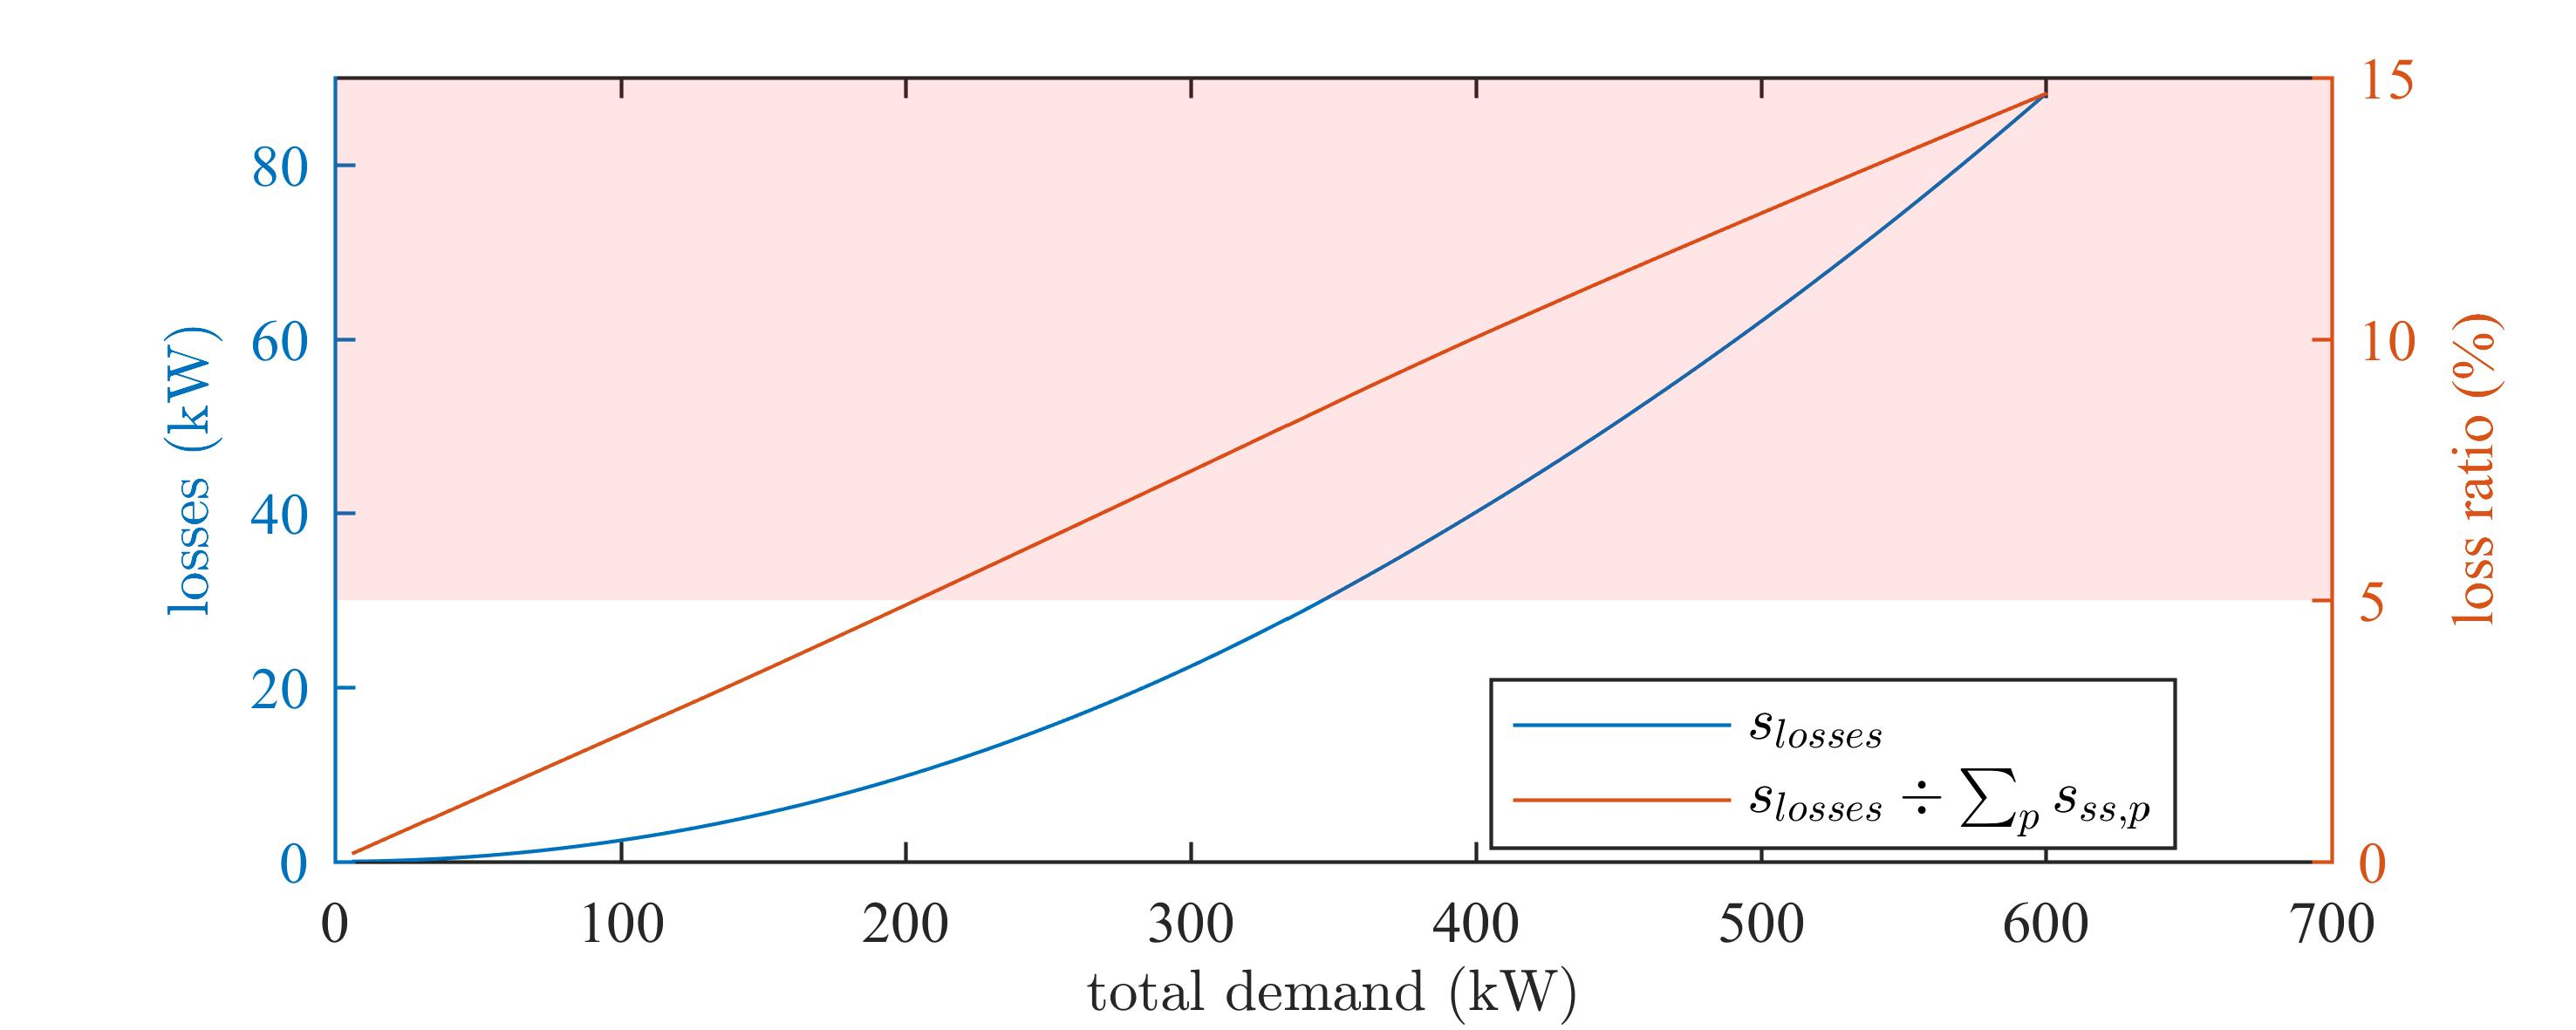
\includegraphics{_chapter1/fig/losses-against-network-demand}
	\caption{Losses against increasing power demand}
	\label{ch1:fig:losses-against-network-demand}
\end{figure}

In Figure \ref{ch1:fig:losses-against-network-demand}, the region where losses exceed 5\% of the total network power is highlighted in red.
These preliminary results were found from power flow simulations.
In reality however, losses cannot be determined this easily.
Therefore, the network losses, $s_{losses}(t)$, are seen as theoretical key network parameters and used in the final cost function $\zeta_\text{losses}(s_{losses}(t))$, which is simply defined as:

\begin{equation}
	\zeta_\text{losses}(s(t)) := |s(t)| 
	\label{ch1:equ:losses}
\end{equation}

